%===============================================
% Setup thư viện
\documentclass{beamer}
\mode<presentation>
\usepackage{hyperref}
\usepackage[utf8]{vietnam}
\usepackage{time}
\usepackage[T5]{fontenc}
\usepackage{latexsym,amsmath,xcolor,multicol,booktabs,calligra}
\usepackage{graphicx,pstricks,listings,stackengine}
\usepackage{Ritsumeikan}
\usepackage{lipsum}
\usepackage{url}
\usepackage{matlab-prettifier}
\usepackage{xsavebox} 
\usepackage{animate}  
\usepackage{MnSymbol}
\usepackage{media9}  
\usepackage{xintexpr}
\usepackage[most]{tcolorbox}
\usepackage{listings}
\usepackage{lstautogobble}
%===============================================
% Setup dữ liệu đề tài
\author{Dương Gia Bảo}
\title{\textbf{Simple SQL Query Tool}}
\subtitle{\textbf{Báo cáo đề tài thử thách}}
\institute{
	TickLab
}
\date{\today}
%===============================================
\setbeamertemplate{navigation symbols}{} % ẩn thanh công cụ
\def\cmd#1{\texttt{\color{red}\footnotesize $\backslash$#1}}
\def\env#1{\texttt{\color{blue}\footnotesize #1}}
\definecolor{deepblue}{rgb}{0,0,0.5}
\definecolor{deepred}{rgb}{0.6,0,0}
\definecolor{deepgreen}{rgb}{0,0.5,0}
\definecolor{halfgray}{gray}{0.55}
\lstset{
	basicstyle=\ttfamily\small,
	keywordstyle=\bfseries\color{deepblue},
	emphstyle=\ttfamily\color{deepred},  
	stringstyle=\color{deepgreen},
	numbers=left,
	numberstyle=\small\color{halfgray},
	rulesepcolor=\color{red!20!green!20!blue!20}
}
%===============================================
% Setup code scroll
\definecolor{codemaincolor}{RGB}{0, 0, 0}
\definecolor{codebackgroundcolor}{RGB}{255, 255, 255}
\definecolor{codekeywordcolor}{RGB}{0, 0, 255}
\definecolor{codestringcolor}{RGB}{163, 21, 21}
\definecolor{codecommentcolor}{RGB}{39, 139, 39}
\definecolor{codeusertypecolor}{RGB}{43, 145, 175}
\lstset {
	basicstyle={\scriptsize \ttfamily \color{codemaincolor}},
	backgroundcolor=\color{codebackgroundcolor},
	autogobble = true,
	tabsize = 2,
	xleftmargin=25pt,
	xrightmargin=0pt,
	aboveskip=0pt, 
	belowskip=0pt, 
	literate=
	% Vần a
	{á}{{\'a}}1
	{à}{{\`a}}1
	{ạ}{{\d a}}1
	{ả}{{\h a}}1
	{ã}{{\~ a}}1
	%
	{Á}{{\'A}}1
	{À}{{\`A}}1
	{Ạ}{{\d A}}1
	{Ả}{{\h A}}1
	{Ã}{{\~ A}}1
	%
	% Vần ă
	{ă}{{\u a}}1
	{ắ}{{\'\abreve }}1
	{ằ}{{\`\abreve }}1
	{ặ}{{\d \abreve }}1
	{ẳ}{{\h \abreve }}1
	{ẵ}{{\~\abreve }}1
	%
	{Ă}{{\u A}}1
	{Ắ}{{\'\ABREVE }}1
	{Ằ}{{\`\ABREVE }}1
	{Ặ}{{\d \ABREVE }}1
	{Ẳ}{{\h \ABREVE }}1
	{Ẵ}{{\~\ABREVE }}1
	%
	% Vần â
	{â}{{\^ a}}1
	{ấ}{{\'\acircumflex }}1
	{ầ}{{\`\acircumflex }}1
	{ậ}{{\d \acircumflex }}1
	{ẩ}{{\h \acircumflex }}1
	{ẫ}{{\~\acircumflex }}1
	%
	{Â}{{\^ A}}1
	{Ấ}{{\'\ACIRCUMFLEX }}1
	{Ầ}{{\`\ACIRCUMFLEX }}1
	{Ậ}{{\d \ACIRCUMFLEX }}1
	{Ẩ}{{\h \ACIRCUMFLEX }}1
	{Ẫ}{{\~\ACIRCUMFLEX }}1
	%
	% Vần đ
	{đ}{{\dj }}1
	{Đ}{{\DJ }}1
	%
	% Vần e
	{é}{{\'e}}1
	{è}{{\`e}}1
	{ẹ}{{\d e}}1
	{ẻ}{{\h e}}1
	{ẽ}{{\~ e}}1
	%
	{É}{{\'E}}1
	{È}{{\`E}}1
	{Ẹ}{{\d E}}1
	{Ẻ}{{\h E}}1
	{Ẽ}{{\~ E}}1
	%
	% Vần ê
	{ê}{{\^e}}1
	{ế}{{\'\ecircumflex }}1
	{ề}{{\`\ecircumflex }}1
	{ệ}{{\d \ecircumflex }}1
	{ể}{{\h \ecircumflex }}1
	{ễ}{{\~\ecircumflex }}1
	%
	{Ê}{{\^E}}1
	{Ế}{{\'\ECIRCUMFLEX }}1
	{Ề}{{\`\ECIRCUMFLEX }}1
	{Ệ}{{\d \ECIRCUMFLEX }}1
	{Ể}{{\h \ECIRCUMFLEX }}1
	{Ễ}{{\~\ECIRCUMFLEX }}1
	%
	% Vần i
	{í}{{\'i}}1
	{ì}{{\`\i }}1
	{ị}{{\d i}}1
	{ỉ}{{\h i}}1
	{ĩ}{{\~\i }}1
	%
	{Í}{{\'I}}1
	{Ì}{{\`I}}1
	{Ị}{{\d I}}1
	{Ỉ}{{\h I}}1
	{Ĩ}{{\~I}}1
	%
	% Vần o
	{ó}{{\'o}}1
	{ò}{{\`o}}1
	{ọ}{{\d o}}1
	{ỏ}{{\h o}}1
	{õ}{{\~o}}1
	%
	{Ó}{{\'O}}1
	{Ò}{{\`O}}1
	{Ọ}{{\d O}}1
	{Ỏ}{{\h O}}1
	{Õ}{{\~O}}1
	%
	% Vần ô
	{ô}{{\^o}}1
	{ố}{{\'\ocircumflex }}1
	{ồ}{{\`\ocircumflex }}1
	{ộ}{{\d \ocircumflex }}1
	{ổ}{{\h \ocircumflex }}1
	{ỗ}{{\~\ocircumflex }}1
	%
	{Ô}{{\^O}}1
	{Ố}{{\'\OCIRCUMFLEX }}1
	{Ồ}{{\`\OCIRCUMFLEX }}1
	{Ộ}{{\d \OCIRCUMFLEX }}1
	{Ổ}{{\h \OCIRCUMFLEX }}1
	{Ỗ}{{\~\OCIRCUMFLEX }}1
	%
	% Vần ơ
	{ơ}{{\ohorn }}1
	{ớ}{{\'\ohorn }}1
	{ờ}{{\`\ohorn }}1
	{ợ}{{\d \ohorn }}1
	{ở}{{\h \ohorn }}1
	{ỡ}{{\~\ohorn }}1
	%
	{Ơ}{{\OHORN }}1
	{Ớ}{{\'\OHORN }}1
	{Ờ}{{\`\OHORN }}1
	{Ợ}{{\d \OHORN }}1
	{Ở}{{\h \OHORN }}1
	{Ỡ}{{\~\OHORN }}1
	%
	% Vần u
	{ú}{{\'u}}1
	{ù}{{\`u}}1
	{ụ}{{\d u}}1
	{ủ}{{\h u}}1
	{ũ}{{\~u}}1
	%
	{Ú}{{\'U}}1
	{Ù}{{\`U}}1
	{Ụ}{{\d U}}1
	{Ủ}{{\h U}}1
	{Ũ}{{\~U}}1
	%
	% Vần ư
	{ư}{{\uhorn }}1
	{ứ}{{\'\uhorn }}1
	{ừ}{{\`\uhorn }}1
	{ự}{{\d \uhorn }}1
	{ử}{{\h \uhorn }}1
	{ữ}{{\~\uhorn }}1
	%
	{Ư}{{\UHORN }}1
	{Ứ}{{\'\UHORN }}1
	{Ừ}{{\`\UHORN }}1
	{Ự}{{\d \UHORN }}1
	{Ử}{{\h \UHORN }}1
	{Ữ}{{\~\UHORN }}1
	%
	% Vần y
	{ý}{{\'y}}1
	{ỳ}{{\`y}}1
	{ỵ}{{\d y}}1
	{ỷ}{{\h y}}1
	{ỹ}{{\~y}}1
	%
	{Ý}{{\'Y}}1
	{Ỳ}{{\`Y}}1
	{Ỵ}{{\d Y}}1
	{Ỷ}{{\h Y}}1
	{Ỹ}{{\~Y}}1
}
\newcommand{\smoothScroll}[5][]{
	\savebox\measBox{\xusebox{#2}}
	\edef\boxwd{\the\wd\measBox}
	\edef\boxht{\the\ht\measBox}
	\edef\boxtht{\the\dimexpr\ht\measBox+\dp\measBox\relax}
	\edef\portht{\the\dimexpr#3\relax}
	\begin{animateinline}[#1,label={#2},width=\boxwd,height=\portht]{#5}
		\multiframe{#4}{
			dRaiseLen=\the\dimexpr-\boxht+\portht\relax+\the\dimexpr(\boxtht-\portht)/
			\numexpr#4-1\relax\relax
		}{
			\begin{minipage}[b][\portht][b]{\boxwd}
				\raisebox{\dRaiseLen}[0pt][0pt]{\xusebox{#2}}
			\end{minipage}
		}
	\end{animateinline}
}
\newsavebox\measBox 
\newcommand{\topScrollButton}[2]{
	\mediabutton[
	jsaction={
		if(event.shift){anim['#1'].pause();anim['#1'].frameNum=0;}
		else try{anim['#1'].frameNum-=#2}catch(e){anim['#1'].frameNum=0;}
	}
	]{\fboxsep=0pt\framebox[\widthof{\xusebox{#1}}][c]{
			\tiny\strut\raisebox{-0.2\height}{$\triangle\triangle\triangle$}}
	}
}
\newcommand{\botScrollButton}[2]{
	\mediabutton[
	jsaction={
		if(event.shift){anim['#1'].pause();anim['#1'].frameNum=anim['#1'].numFrames-1;}
		else try{anim['#1'].frameNum+=#2}catch(e){anim['#1'].frameNum=anim['#1'].numFrames-1;}
	}
	]{\fboxsep=0pt\framebox[\widthof{\xusebox{#1}}][c]{
			\tiny\strut\raisebox{0.1\height}{$\triangledown\triangledown\triangledown$}}
	}
}
	\lstnewenvironment{codescroll}[4][style=Matlab-editor]
	{\lstset{#1}\xlrbox{#2}\noindent\minipage{\linewidth}}
	{\endminipage\endxlrbox
		\def\lnsperframe{28}
		\def\lnht{5}
		\def\lnspersec{3}
		\def\htpercentage{\xintthefloatexpr #4 / \lnsperframe \relax}
		\def\steps{\xintexpr #3 - #4 + 1 \relax}
		\def\viewportheight{\xinttheiexpr (#3 + 1)  * \lnht \relax}
		\def\btnstep{\xintthefloatexpr \viewportheight / \steps \relax}
		\def\stepspersec{\xintthefloatexpr \lnspersec * \btnstep \relax}
		\topScrollButton{#2}{\btnstep}\\
		\smoothScroll{#2}{\htpercentage\textheight}{\viewportheight}{\stepspersec}\\
		\raisebox{2ex}{\botScrollButton{#2}{\btnstep}}
	}
%===============================================
\begin{document}
	\begin{frame}
		\titlepage
		\begin{figure}[htpb]
			\begin{center}
				
\includegraphics[scale=0.2]{ticklablogo.png}
			\end{center}
		\end{figure}
	\end{frame}

	
	\begin{frame}
		\tableofcontents[sectionstyle=show,subsectionstyle=show/shaded/hide,subsubsectionstyle=show/shaded/hide]
	\end{frame}
	
	\section{Mở đầu}
	
	\begin{frame}
		Mục tiêu:
		\begin{itemize}
			\item Xây dựng công cụ truy vấn CSV sử dụng cú pháp SQL
			\item Nâng cao khả năng lập trình với C++
		\end{itemize}
		Nội dung:
		\begin{itemize}
			\item Thiết kế và xây dựng chương trình exql
			\item Bộ phân tích cú pháp truy vấn
			\item Đọc và xử lý tệp CSV
		\end{itemize}
		\begin{figure}
			\centering
			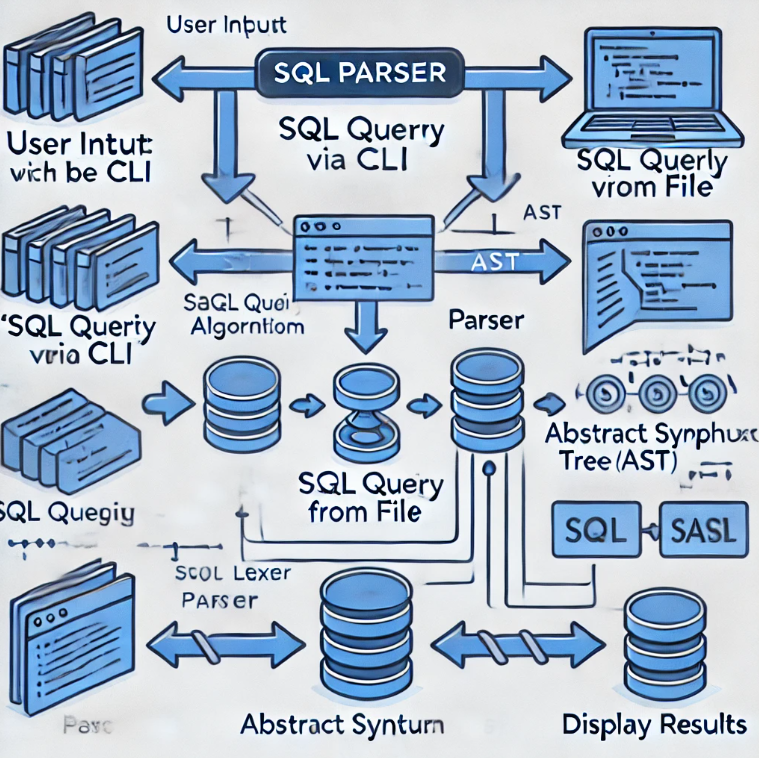
\includegraphics[width=0.4\linewidth]{parser}
			\label{fig:parser}
		\end{figure}
		
	\end{frame}
	
	
	\section{Timelines}
	
	\subsection{SQL Lexer}
	
	\begin{frame}	
		\begin{tcolorbox}[colback=yellow!10!white,colframe=red!75!black,title= Mục tiêu]
		Triển khai giao diện dòng lệnh (CLI) và SQL Lexer cho dự án.
		\end{tcolorbox}
		Các bước thực hiện:
		\begin{itemize}
			\item Định nghĩa các token: 
			\begin{itemize}
				\item[$\checkmark$] Tạo một liệt kê cho các loại token (từ khóa, định danh, literal, toán tử, dấu phân cách, khoảng trắng).
			\end{itemize}
			\item Triển khai các hàm phân tích token
			\begin{itemize}
				\item[$\checkmark$] Từ khóa và Định danh: Phân tích các từ khóa SQL như SELECT, FROM và các định danh (tên cột và bảng).
				\item[$\checkmark$] Literal: Xử lý các literal kiểu chuỗi và số.
				\item[$\checkmark$]  Xử lý các toán tử.
			\end{itemize}
		\end{itemize}
				
	\end{frame}
	\begin{frame}
		\begin{itemize}
			\item Xử lý lỗi
			\begin{itemize}
				\item[$\checkmark$] Triển khai xử lý lỗi cho các token không được hỗ trợ hoặc không mong muốn.
				\item[$\checkmark$] Định nghĩa các loại lỗi và một lớp để theo dõi vị trí và loại lỗi trong truy vấn SQL.
			\end{itemize}
			\item Kiểm thử
			\begin{itemize}
				\item[$\checkmark$] Kiểm thử lexer với các truy vấn SQL khác nhau để đảm bảo nó có thể phân tích đúng các token.
				\item[$\checkmark$] Đảm bảo lexer xử lý đúng các token hợp lệ và đưa ra lỗi thích hợp cho các đầu vào không hợp lệ.
			\end{itemize}
		\end{itemize}
	\end{frame}
	
	\subsection{SQL Parser}
	\begin{frame}
		\begin{tcolorbox}[colback=yellow!10!white,colframe=red!75!black,title= Mục tiêu]
			Xây dựng trình phân tích cú pháp SQL để chuyển đổi luồng mã thông báo thành Cây cú pháp trừu tượng (AST), thể hiện cấu trúc của truy vấn SQL theo cách có ý nghĩa.
		\end{tcolorbox}
		\begin{itemize}
			\item Trong giai đoạn Lexer trước đó, chúng ta đã biến chuỗi truy vấn thô thành một chuỗi các token. Tuy nhiên, việc nhận dạng token không đảm bảo rằng chuỗi này là một truy vấn hợp lệ và có ý nghĩa.
			\item SQL Parser đảm bảo rằng chuỗi token tuân theo các quy tắc ngữ pháp của ngôn ngữ truy vấn CSV, xây dựng một biểu diễn cú pháp dưới dạng Abstract Syntax Tree (AST).
		\end{itemize}
	\end{frame}
	
	\begin{frame}
		Các bước thực hiện:
		\begin{itemize}
			\item Định nghĩa cấu trúc dữ liệu cho AST:
			\begin{itemize}
				\item[$\checkmark$] SQL Statements.
				\item[$\checkmark$] Biểu thức (Expressions).
			\end{itemize}
			\item Định nghĩa Parser:
			\begin{itemize}
				\item[$\checkmark$] Xây dựng các phương thức như parse$\_$statement() và parse$\_$expression().
			\end{itemize}
			\item Xử lý lỗi.
			\item Kiểm thử.
		\end{itemize}
	\end{frame}
	
	\subsection{Handle file}
	\begin{frame}
		\begin{tcolorbox}[colback=yellow!10!white,colframe=red!75!black,title= Mục tiêu]
			Xây dựng chức năng xử lý tệp cho SQL Parser, cho phép người dùng nhập truy vấn từ tệp và thực thi chúng một cách hiệu quả.
		\end{tcolorbox}
		\begin{figure}
			\centering
			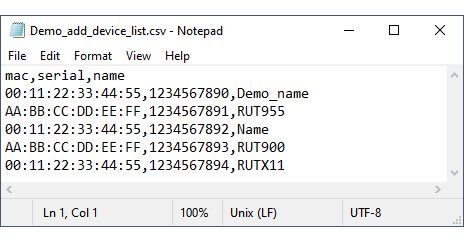
\includegraphics[width=0.7\linewidth]{csvfile}
			\label{fig:csvfile}
		\end{figure}
	\end{frame}
	
	\begin{frame}
		Các bước thực hiện:
		\begin{itemize}
			\item Định Nghĩa Chức Năng Đọc Tệp.
			\item Xử Lý Tệp Đầu Vào.
			\item Phân Tích Truy Vấn:
			\begin{itemize}
				\item[$\checkmark$] Sau khi đọc được nội dung từ tệp hoặc chuỗi đầu vào, sử dụng Parser để phân tích truy vấn và xây dựng AST. Đảm bảo xử lý các trường hợp lỗi nếu có vấn đề trong quá trình phân tích.
			\end{itemize}
			\item Xử Lý Kết Quả.
		\end{itemize}
	\end{frame}
	
	\section{Kết luận}
	\begin{frame}
		Hoàn thành:
		\begin{itemize}
			\item Xử lý Lexer
			\item Phân tích Parser Statement
			\item Handle file
		\end{itemize}
		Chưa hoàn thành:
		\begin{itemize}
			\item Phân Tích Parser Expression
			\item Handle Error trong Parser
			\item Xử Lý Parser Statement trên nhiều dòng
		\end{itemize}
	\end{frame}
	
	\begin{frame}
		\begin{center}
			{\Huge\calligra Thank You}
		\end{center}
	\end{frame}
	
\end{document}